\documentclass[class=book, crop=false, oneside]{standalone}
\usepackage[subpreambles=true]{standalone}

\usepackage{../../style}

\graphicspath{{./assets/images/}}
\newmintinline{asm}{}

% arara: pdflatex: { synctex: yes, shell: yes }
% arara: latexmk: { clean: partial }
\begin{document}
\chapter{Central Processing Unit}

In questo capitolo andremo ad analizzare come il nostro processore elabora ed esegue le istruzioni che gli arrivano dai programmi Assembly; in particolare ci baseremo ancora su MIPS, in quanto super regolare e particolarmente utile a scopo didattico.\\

\section{Introduzione}
Per come è stato progettato MIPS, le istruzioni presentano dei tratti comuni;in particolare le prime due fasi del ciclo della CPU (vedi~\ref{subsec:cpu}), ossia il prelievo dell'istruzione e la lettura dei valori dei registri operandi sono comuni a ogni istruzione.\\
Noi in particolare, dopo aver spiegato i vari elementi che concorrono a far funzionare tutta la baracca, andremo ad analizzare le istruzioni aritmetico-logiche, quelle di accesso alla memoria e quelle di salti, dal momento che tutte le altre si implementano con tecniche simili.

\section{Arithmetic-Logic Unit}
A eccezione di \mintinline{asm}{j}, tutte le istruzioni MIPS fanno uso di \emph{arithmetic-logic unit} (ALU per gli amici), una rete logica combinatoria abbastanza complessa preposta all'esecuzione di tutti calcoli di cui abbiamo bisogno; sostanzialmente, è un’unione di blocchi fondamentali che fanno operazioni su singoli bit.\\
Al di là delle operazioni puramente aritmetiche (per le quali lo scopo di ALU è ovvio), viene usato nelle operazioni di accesso alla memoria (\mintinline{asm}{sw} e \mintinline{asm}{lw}) per il calcolo degli indirizzi e dalle operazioni di salto condizionato per effettuare i confronti; successivamente, ognuna di queste tre categorie differisce. \\

\section{Il datapath}
Il \emph{datapath} è quella parte del processore attraverso cui passano le istruzioni; è letteralmente un percorso da seguire ogniqualvolta si voglia esegire una qualsiasi istruzione.

\subsection{Struttura del datapath}
\begin{figure}[H]
	\centering
	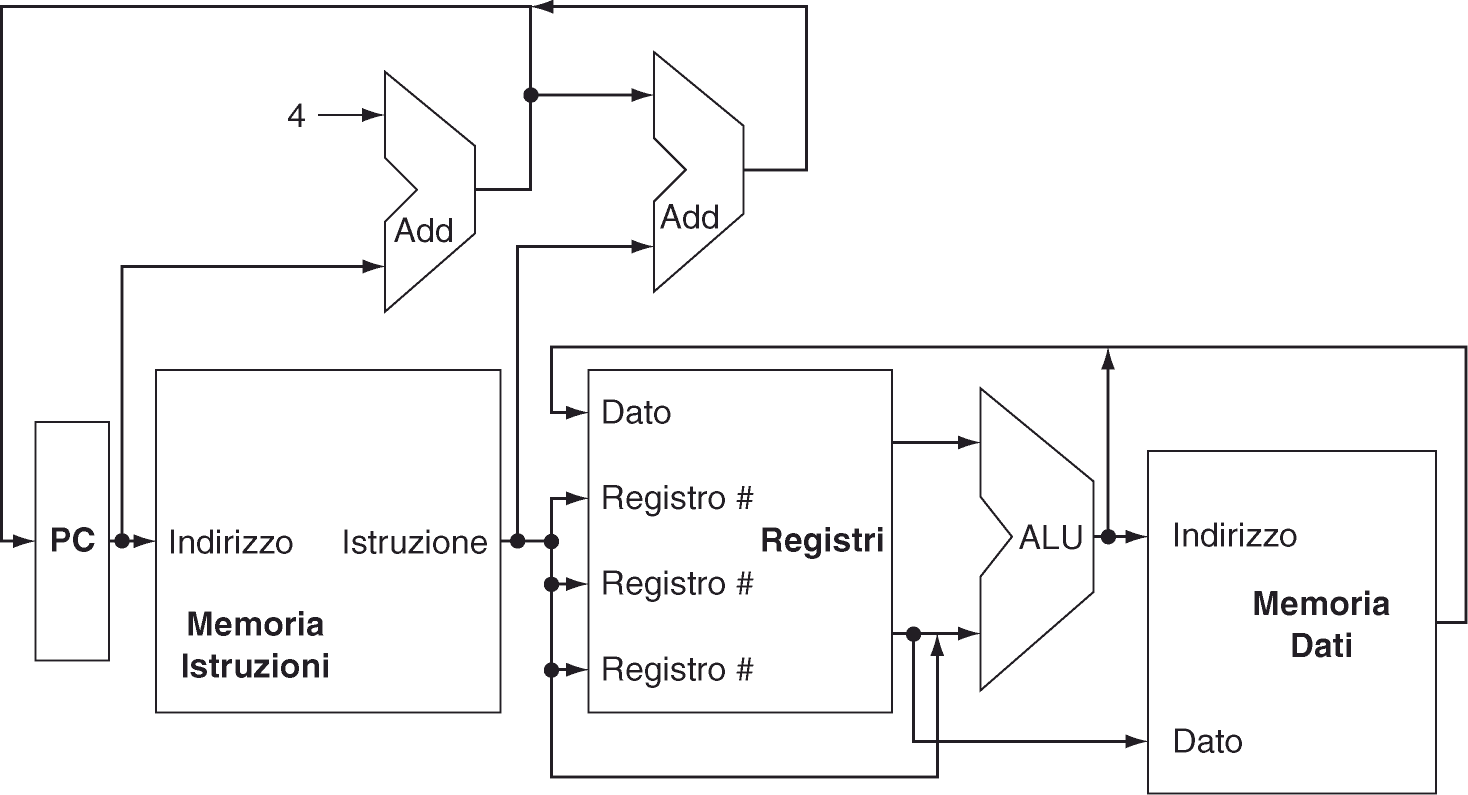
\includegraphics[width=0.9\textwidth,keepaspectratio]{datap_1}
	\caption{Schema base del datapath}
\end{figure}
Il datapath si compone essenzialmente di 5 fasi:
\begin{enumerate}
  \item assumendo che il programma sia già stato caricato in memoria (secondo le modalità viste nel capitolo~\ref{ch:tool}), in questa fase viene prelevata l'istruzione da eseguire e viene spacchettata nei vari campi;
  \item i registri interessati all'esecuzione vengono caricati nel \emph{banco dei registri}; se l'istruzione è di tipo R, gli indirizzi dei registri sono contenuti nel corpo dell'istruzione;
  \item a questo punto la ALU esegue i calcoli opportuni, ottenendo il valore (o l’indirizzo) desiderato;
  \item i risultati ALU vengono utilizzati per salvare (o prelevare) in memoria dati un dato, o per memorizzare un registro;
  \item si incrementa il program counter per mezzo di una ALU dedicata (di fatto, un addizionatore), e una successiva ALU calcola l’indirizzo verso cui mi dovrò spostare in caso di salti incondizionati;
\end{enumerate}

\subsection{Il ruolo del multiplexer}
La  figura però è incompleta; manca qualcosa che dica ai blocchi cosa fare in caso di punti di decisione (momenti in cui i segnali arrivano da due diverse sorgenti e bisogna sceglierne una), come ad esempio l'incremento del program counter: normalmente, il suo valore proviene dall'addizionatore (e punta quindi alla word successiva a quella appena letta), ma in caso di salto l'indirizzo viene calcolato dallo spiazzamento contenuto nell'istruzione.\\
Altro esempio: a seconda della tipologia di istruzione il secondo operando della ALU potrà provenire o dal banco dei registri (per le istruzioni R) o dal codice dell'istruzione stessa (per le istruzioni I).\\
Ed è qui che ci viene in soccorso il \emph{multiplexer} che, come già detto in~\ref{subsec:multi}, è un circuito combinatorio che prende in input due segnati e decide quale di essi debba andare in output sulla base di un terzo segnale di controllo (un po' come un vigile che decide quale macchina far passare).
\begin{figure}[H]
	\centering
	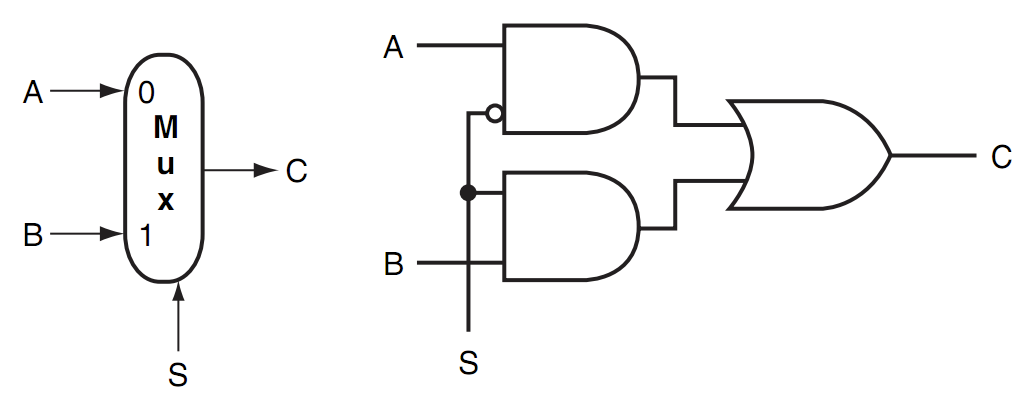
\includegraphics[width=0.8\textwidth,keepaspectratio]{multi}
	\caption{Schema di un multiplexer}
\end{figure}
\paragraph{Altri elementi}
Oltre ai multiplexer, ci sono altri elementi che concorrono alla soluzione dei punti di decisione. Ad esempio le ALU ha diversi ingressi per decidere quale operazione effettuare e il banco dei registri ha delle porte per decidere se scrivere o meno un registro, e la memoria dati ha degli espedienti per decidere se effettuare lettura o scrittura.\\
E chi stabilisce queste cose, oltre a settare il segnale del selettore dei vari multiplexer?  È presto detto, l’unità di controllo!\\

\section{La control unit}
La \emph{control unit} funge da vero e proprio "direttore d'orchestra" per il processore, stabilendo il valore \(S\) dei vari multiplexer e andando a sciogliere le questioni dei punti di decisione.
\begin{figure}[H]
	\centering
	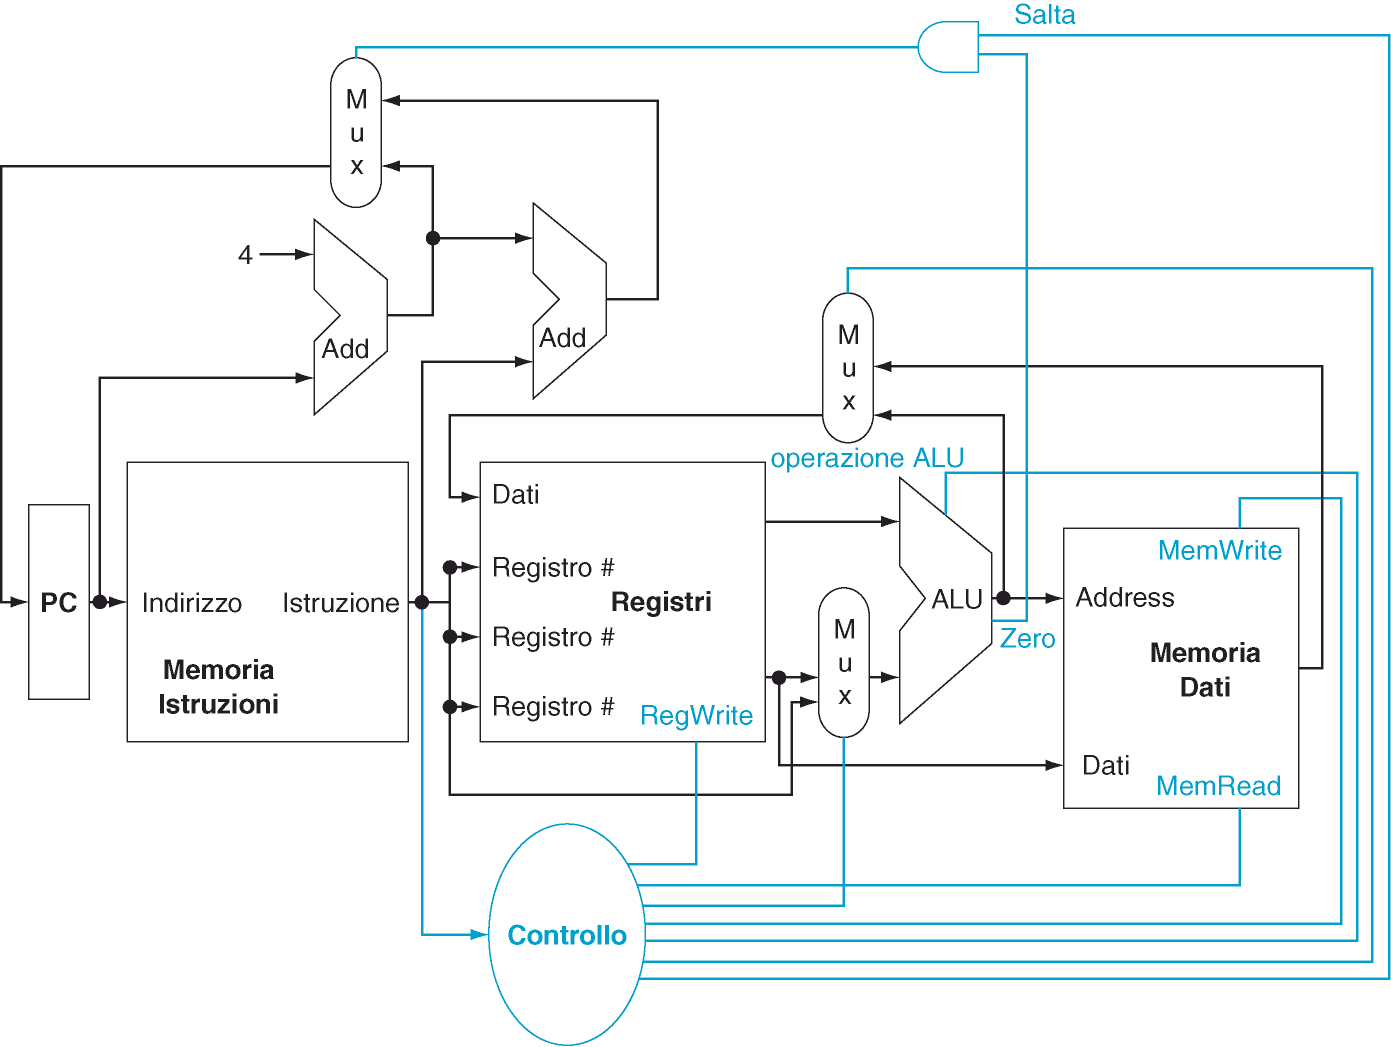
\includegraphics[width=0.9\textwidth,keepaspectratio]{datap_2}
	\caption{Schema di datapath e control unit}
\end{figure}
La figura è molto complessa, andiamo ad analizzarla con ordine.
\begin{itemize}
	\item Innanzitutto notiamo il multiplexer prima del pc: questo gestisce la scelta su come viene aggiornato il pc, se secondo il valore del primo o del secodno addizionatore. Per settare il valore \(S\) viene utilizzata una porta AND, il cui primo input arriva direttamente dalla control unit, mentre il secondo viene fornito dalla ALU (\emph{zero}) (come straminchia riconosce se stiamo facendo un salto oppure no?).
	\item Vediamo un secondo multiplexer che indica se memorizzare nel registro di destinazione un dato da ALU o dalla memoria
	\item Abbiamo un  ultimo multiplexer che precede il caricamento del secondo operando nell'ALU: dalla control unit arriverà l'indicazione per scegliere di caricare un registro (nelle istruzioni R) o una costante (per quelle I).
	\item Poi vediamo un segnale per la ALU: esso consiste di un bus di più bit per comunicare all'unità quale operazione eseguire.
	\item Alla memoria dati invece arrivano i segnali \emph{MemWrite} e \emph{MemRead}, che indicano alla memoria dati  la rispettiva operazione.
	\item \emph{RegWrite} dice di scrivere il registro (decisamente da approfondire).
\end{itemize}

Questa è la rappresentazione di MIPS, che è una ISA RISC; inutile dire che gli schemi di funzionamento che stanno alla base di architetture CISC sono incredibilmente di così.

\section{La temporizzazione}
A questo punto abbiamo moltissimi segnali che viaggiano nel processore, sincronizzati dal clock. Per semplicità assumiamo che tutte le istruzioni vengano eseguite con un ipotetico singolo colpo di clock lungo abbastanza.

\subsection{Breve riepilogo sulle reti logiche}
Circuiti come i multiplexer visti prima sono detti \emph{reti combinatorie} e producono un output secondo una funzione statica dell'input, senza memoria dei cambiamenti.\\
Ma è chiaro che elementi come i registri e le memorie (detti elemtni "di stato") necessitano di tenere traccia dei cambiamenti subiti, e a questo si può ovviare con \emph{reti sequenziali}, dove l'output dipende dalla storia (sequenza) degli input precedenti.\\
Gli elementi di stato hanno almeno due ingressi:
\begin{itemize}
	\item valore da immettere nello stato;
	\item clock atto a sincronizzare le transizioni.
\end{itemize}

\paragraph{Flip-flop}Il \emph{flip-flop D-latch} è l’elemento base per memorizzare un bit, e registri sono di fatto vettori di vettori di 32 di questi circuiti. I dettagli su~\ref{subsec:latch}.

\subsection{Gestione della temporizzazione}
Avere un clock regolare ci permette di ottenere indicazioni precise sulla sequenza di operazione svolte e avere sempre ragione di quale istruzione è avvenuta prima o dopo di un determinato colpo di clock. La metodologia di temporizzazione ci dà quindi indicazioni precise rispetto alla possibilità di letura/scrittura dei segnali rispetto al clock, e i dati presi dagli elementi di stato sono sempre relativi ai cicli precedenti. Vediamo uno schema di come viene gestita la cosa:
\begin{figure}[H]
	\centering
	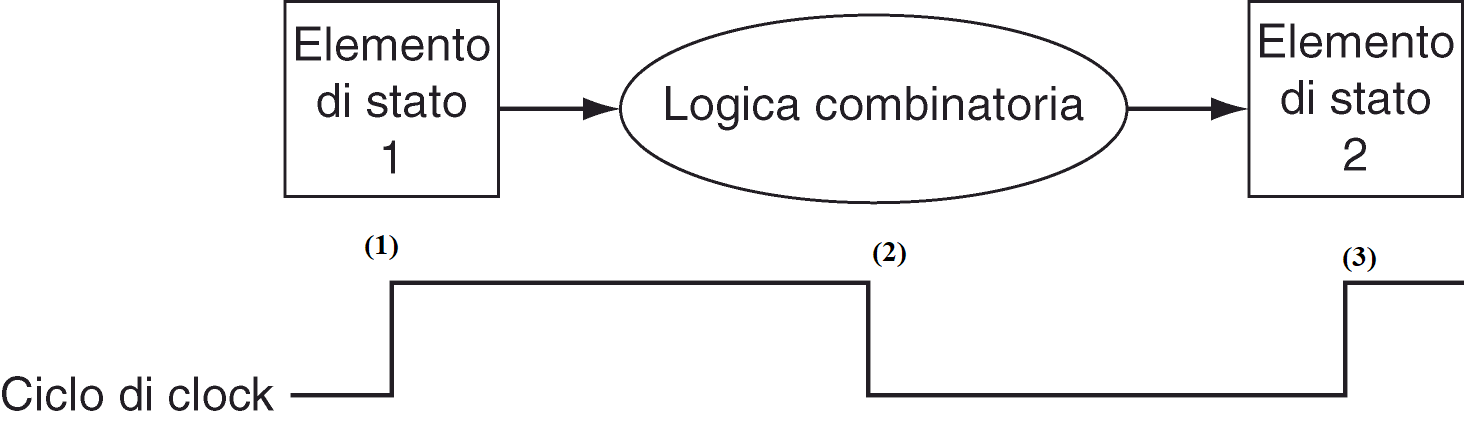
\includegraphics[width=0.6\textwidth,keepaspectratio]{clock}
\end{figure}
\begin{enumerate}
	\item l'elemento di stato 1 viene aggiornato a un determinato tempo \(t\);
	\item il valore passa attraverso a una qualsiasi rete combinatoria;
	\item il valore arriva all'elemento di stato 2 al tempo \(t + T\).
\end{enumerate}
Il tempo \(T\) di clock deve naturalmente essere tale da dare tempo ai valori di attraversare i vari circuiti combinatori; inoltre questa sorta di spiazzamento (si può dire?) del clock ci permette di regolarizzare quelli che altrimenti diventerebbero dei cicli di retroazione assolutamente non predicibili.
\begin{figure}[H]
	\centering
	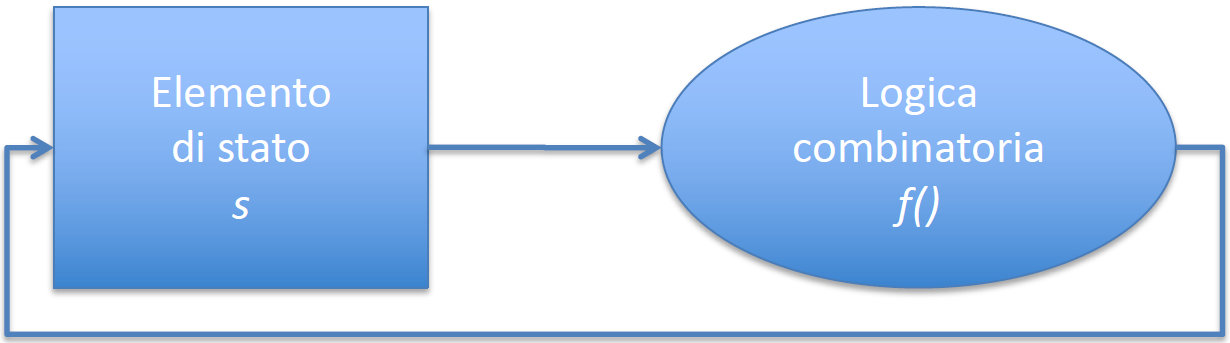
\includegraphics[width=0.5\textwidth,keepaspectratio]{retroaz}
\end{figure}
Se non avessimo una metodologia di temporizzazioneprecisa avremmo che \(s = f(s)\), che risulta una cosa non prevedibile. Grazie alla temporizzazione sensibile al clock possiamo ottenere un andamento del tipo: \(s(t + T) = f(s(t))\), decisamente più regolare ed efficiente per noi.

\section{Elaborazione delle istruzioni}
Prima di addentrarci nel dettaglio dell'esecuzione di alcuni tipi di istruzioni, passiamo in rassegna le varie componenti che servono alla realizzazione di un datapath:
\begin{figure}[H]
	\centering
	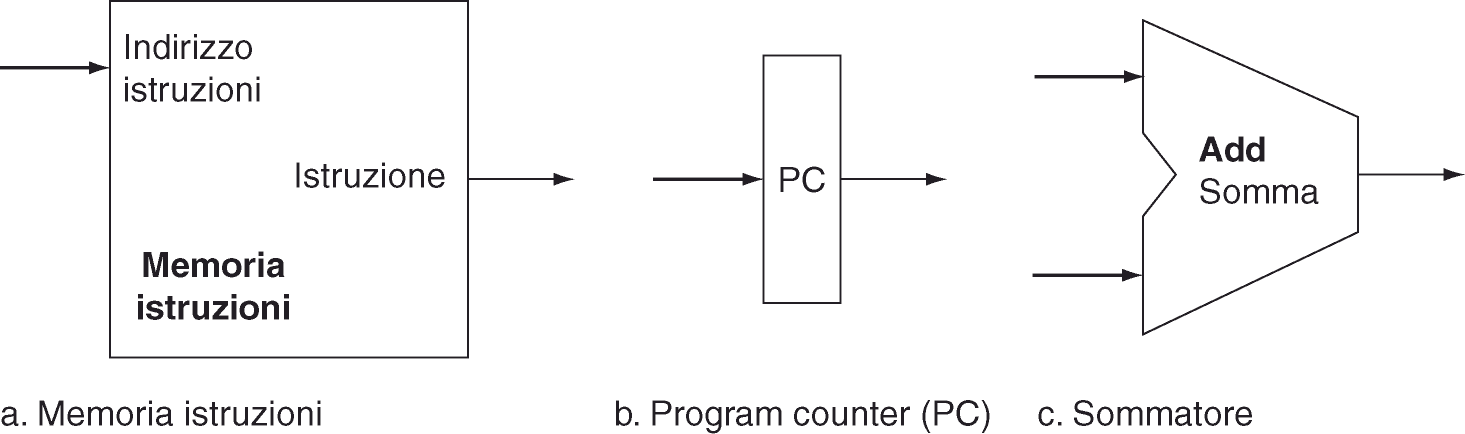
\includegraphics[width=0.9\textwidth,keepaspectratio]{datap_3}
\end{figure}
Ricordiamo che il sommatore (o addizionatore) è una ALU specializzata alla sola operazione di incremento del program counter.\\
A questo punto la fase di fetch, ricordiamolo, prevede il prelievo dell'istruzione dal pc, il trasferimento della stessa agli elementi proposti all'esecuzione e infine l'incremento del program counter.
\subsection{Istruzioni R}
Iniziamo con un’istruzione di tipo R, come potrebbe essere
\begin{minted}[linenos]{asm}
add $t0, $s1, $s2
\end{minted}
la quale, come sappiamo, ha questo tipo di mapping:
\begin{figure}[H]
	\centering
	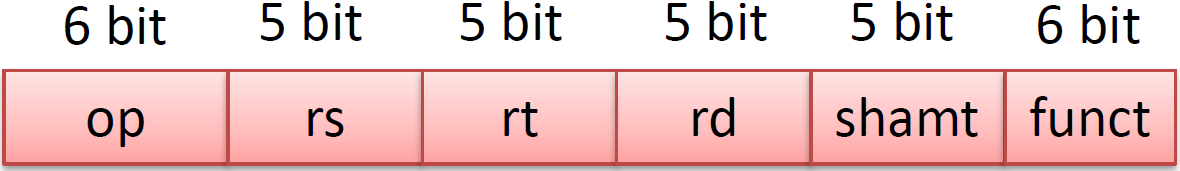
\includegraphics[width=0.5\textwidth,keepaspectratio]{mappatura.png}
\end{figure}
Per effettuare questa operazione ho bisogno di due blocchi funzionali che vano ad aggiungersi ai tre di base che abbiamo visto prima.
\begin{figure}[H]
	\centering
	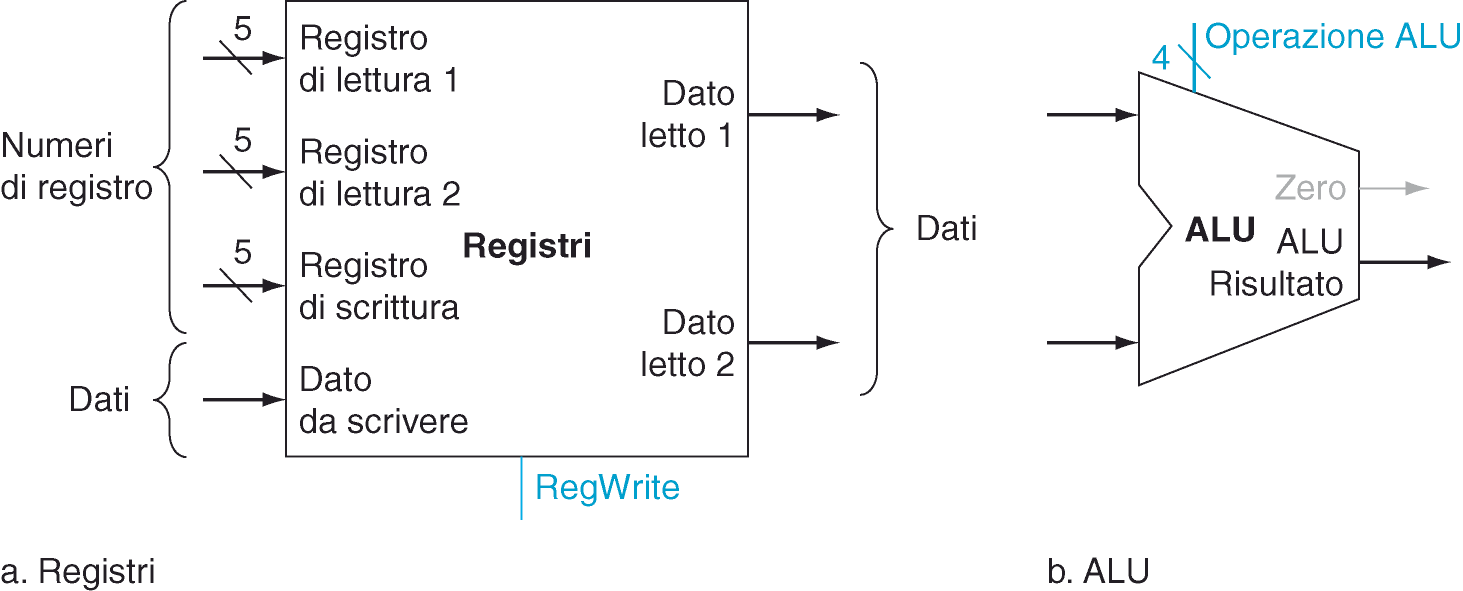
\includegraphics[width=0.8\textwidth,keepaspectratio]{R_ex.png}
\end{figure}
\begin{itemize}
	\item Il primo blocco è il \emph{banco dei registri}, una struttura con 3 bus da 5 bit ciascuno in cui vengono caricati i registri da operare; per decidere se dovrò leggere o scrivere un determinato registro viene impiegato il controllo RegWrite, gestito direttamente dalla control unit.
	\item Il secondo blocco di cui abbiamo bisogno è la ALU di cui prima abbiamo tanto parlato. Questa presenta due controlli, uno di questi è il bus che arriva dal corpo dell'istruzione e indica qual è l'operazione da svolgere, mentre il secondo è il settaggio \emph{zero} qualora il risultato dell'operazione fosse effettivamente 0; questo valore viene poi mandato alla porta AND che decide il segnale di controllo per il multiplexer preposto alla scelta del blocco d'incremento del program counter.
\end{itemize}

\subsection{Istruzioni di accesso alla memoria}
Adesso andiamo ad analizzare le seguenti istruzioni sulla memoria:
\begin{minted}[linenos]{asm}
lw $t0, offest($t2)
sw $t0, offest($t2)
\end{minted}
Ricordiamo che presentano la seguente mappatura:
\begin{figure}[H]
	\centering
	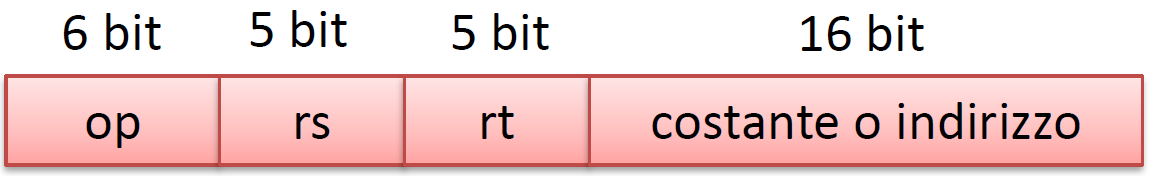
\includegraphics[width=0.5\textwidth,keepaspectratio]{I.png}
\end{figure}
In entrambi i casi avremo bisogno di calcolare l'indirizzo in memoria dato da \register{\$t2} e dallo spiazzamento (register file wtf?), per cui ci servirà nuovamente una ALU.
\begin{figure}[H]
	\centering
	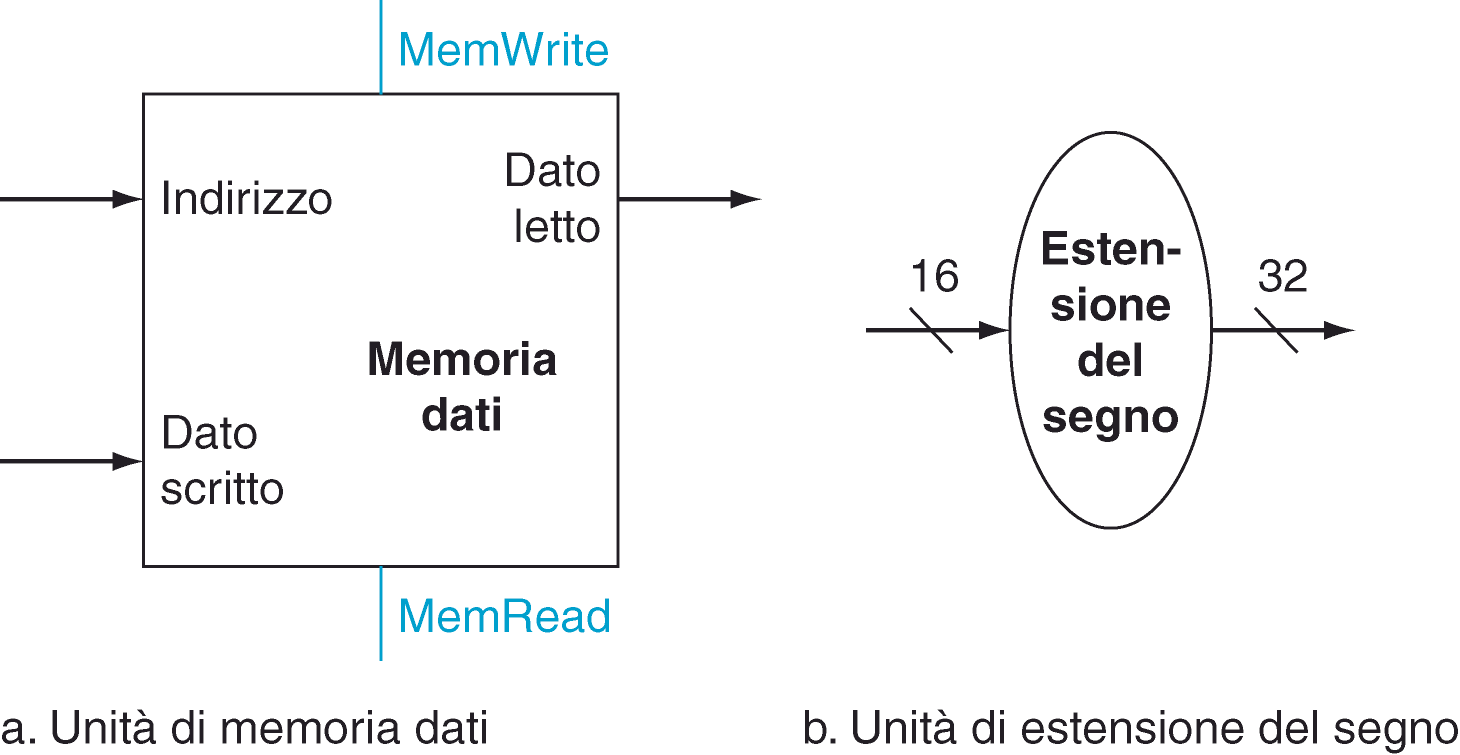
\includegraphics[width=0.65\textwidth,keepaspectratio]{MemAccess.png}
\end{figure}
\begin{itemize}
	\item Naturalmente avremo bisogno di una \emph{memoria dati}, dove eventualmente potremo memorizzare i dati di \mintinline{asm}{sw};
	\item notiamo inoltre che abbiamo bisogno di due segnali di controllo appositi per indicare se l'operazione da eseguire è di lettura o scrittura;
	\item in ultimo, osserviamo che l'offest viene memorizzato in un campo a 16 bit, che potrebbe essere necessario estendere a 32 bit replicando per 16 volte il bit di segno: per questo abbiamo bisogno di un blocco funzionale apposito.
\end{itemize}

\subsection{Istruzioni di salto condizionato}
Andiamo ora a vedere la seguente istruzione:
\begin{minted}[linenos]{asm}
beq $t1, $t2, offset
\end{minted}
Ovviamente anche qui bisogna sommare l'offset, per cui di nuovo necessitiamo di una ALU, ma osserviamo due cose: sappiamo che il pc viene incrementato di 4 byte ogni ciclo, per cui quando effetuiamo un salto andiamo a riferire l'offset al pc già incrementato; inoltre MIPS shifta automaticamente a sinistra di 2 bit, in modo da ragionare sempre in words ed espandere in numero di indirizzi raggiungibili.
\begin{figure}[H]
	\centering
	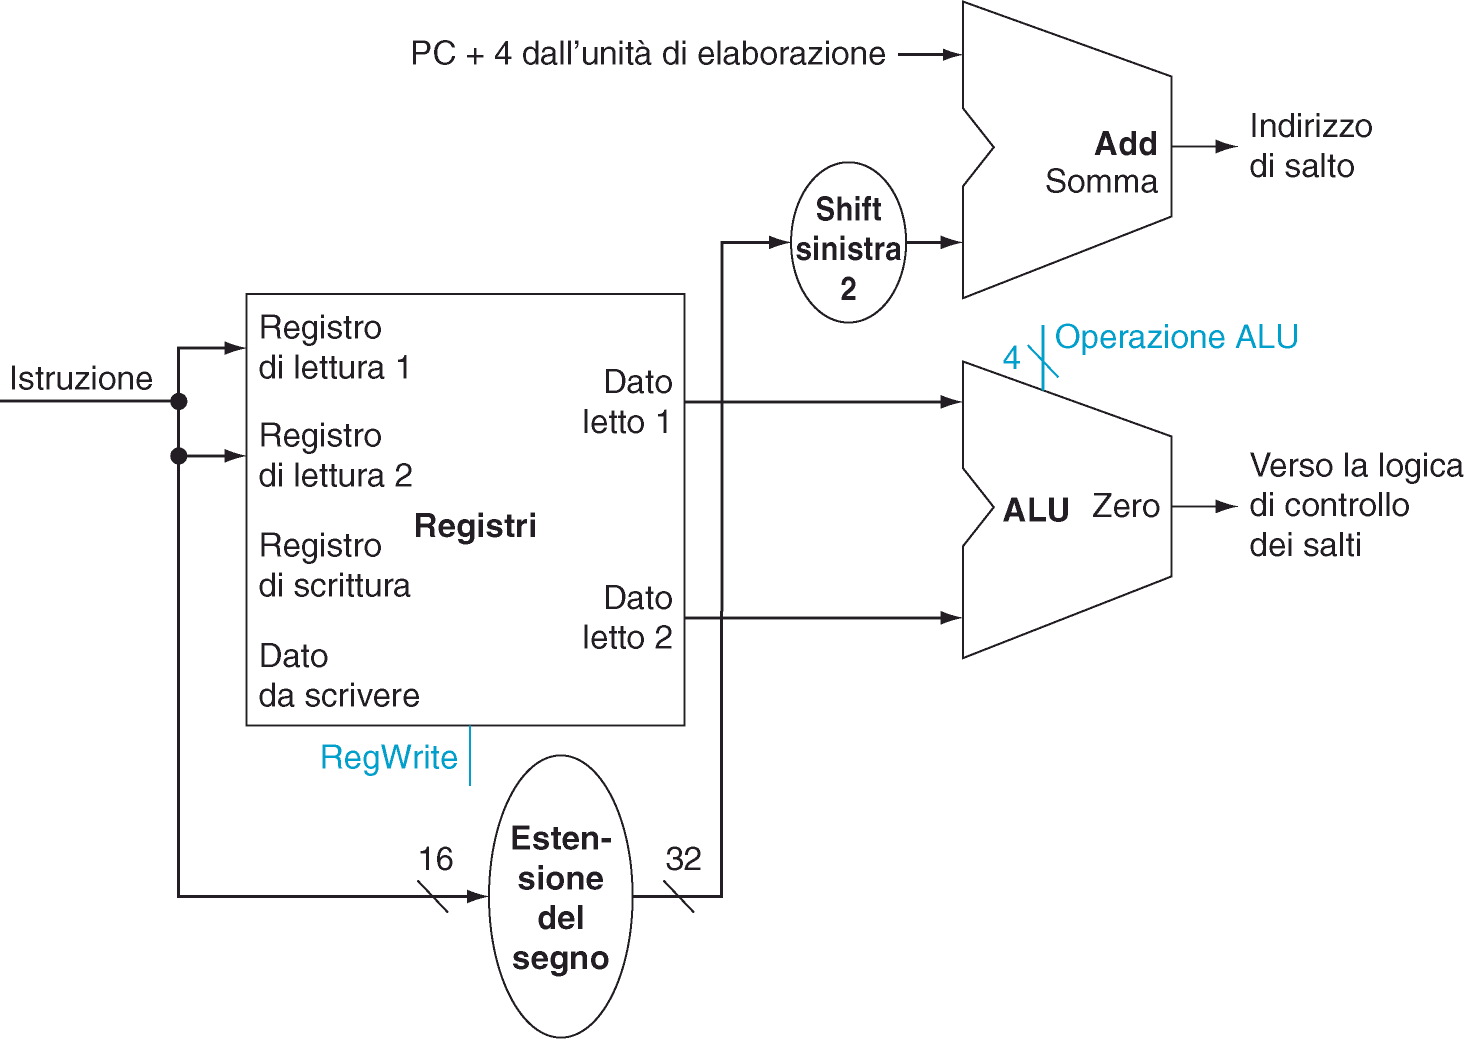
\includegraphics[width=0.7\textwidth,keepaspectratio]{jump.png}
\end{figure}
\begin{itemize}
	\item Notiamo una prima ALU preposta al calcolo dell'indirizzo di salto da comunicare al program counter;
	\item La seconda ALU effettua una sottrazione fra u due registri e se il risultato è 0 (e quindi i due sono uguali) lo comunica alla porta AND che successivamente comunica col multiplexer dell'incremento.
\end{itemize}

\end{document}
